\section{Experiment 1}
\label{Exp1}

\subsection{Methods}
\label{Methods1}
\subsubsection{\large{\emph{Participants}}}
\label{Participants1}

\noindent
Participants were 18-25 years of age, had normal or corrected-to-normal vision, and did not have any learning or reading impairments. The study was run online through Prolific (\cite{Prolific}), and there were no restrictions on participants' spoken languages, other than requiring English fluency. To determine the sample size, we ran a simulation-based power analysis. We accounted for 20 items per condition (see below), a 10\% difference in responses between conditions, 10\% subject intercept variability, 10\% subject slope variability, and 15\% overall noise. The effect size was set to 5\% above chance (see, for example, \textcite{Onnis2018}, with accuracy in an implicit statistical learning task at 7\% above chance). Running 500 simulations, the model estimated that it would be necessary to recruit 200 participants for this effect to be statistically significant in 95\% of simulations.

\subsubsection{\large{\emph{Stimuli}}}
\label{Stimuli1}

\noindent % Characters
Two chunks of characters formed each word in the experiment. However, given the potentially very wide linguistic background of participants, random assemblies of Latin characters might be meaningful in one of the participants' languages (e.g. ``akcja'' is meaningless in English, but is the Polish word for ``action''). This is of particular importance, since evidence shows that a participant's language background and experience influence the processing of new artificial linguistic stimuli (\cite{Siegelman2018}; \cite{Weiss2020}), and new statistical structures are not learned in this situation (\cite{Lelonkiewicz2022}). Should some learning occur, any new regularities placed on known lexical tokens would interact with participants' existing representations (\cite{Frost2019}), and would be an additional confound. This risk was eliminated through the use of the BACS-1 font created by \textcite{Vidal2017} for psycholinguistic studies (see \autoref{BACS1_example}).

\begin{figure}[!htbp]
    \begin{center}
        
\includegraphics[width=0.6\textwidth]{Figures/BACS1_example.png}
    \end{center}
    \caption[]{Example of a word in the BACS-1 font (\cite{Vidal2017}), composed of a stem and a suffix.}
    \label{BACS1_example}
\end{figure}

% Morphemes
In order to generate artificial languages that are as faithful as possible to real-world language structures, these character chunks were organised as morphemes; similarly to many language systems, the words presented to participants in the present experiment were the assembly of two such morphemes/character chunks (see \autoref{BACS1_example}). To ensure that participants were segmenting words according to the morphemes instead of relying on a stable boundary between stem and suffix, stems were 4 or 5 characters long and suffixes 3 or 4 characters long, thereby forming words 7 to 9 characters long. For each participant, 20 stems and 10 suffixes were randomly generated. We dubbed these chunks ``stems'' and ``suffixes'' only based on their distributional properties (e.g. affixes were more frequent and showed up in several different words; see below for details): there was no meaning or syntax in the present experiment, so no stem-affix asymmetry was present in those domains, as would of course happen in real language. Ten stems and five suffixes were then allocated to each of the two stimuli categories, representing two fictional ``languages''. As the morphemes used some of the same BACS-1 characters, these languages were visually indistinguishable. This is also an aspect found in natural languages, such as those using the Latin alphabet.

% Words
Within each language, all stems were assembled with all suffixes, forming congruent strings (from now on, ``words''; see \autoref{Testing_structure}). Of these 50 words, 40 were shown as training items, while 10 were kept as testing items. Therefore, throughout the entire set of 80 training words, each stem was present 4 times (stem frequency in training = 0.05) and each suffix was present 8 times (suffix frequency in training = 0.1). The remaining 10 words from each language were taken as congruent testing items. Alongside these, the stems from each language were combined with suffixes from the other language to form 20 incongruent items (see combinations made with dashed lines in \autoref{Testing_structure}). These 40 items were therefore named the \textbf{two-morpheme} (``2M'') testing condition, with each stem being used twice (stem frequency in 2M = 0.05), and each suffix four times (suffix frequency in 2M = 0.1).

\begin{figure}[!htbp]
    \begin{center}
        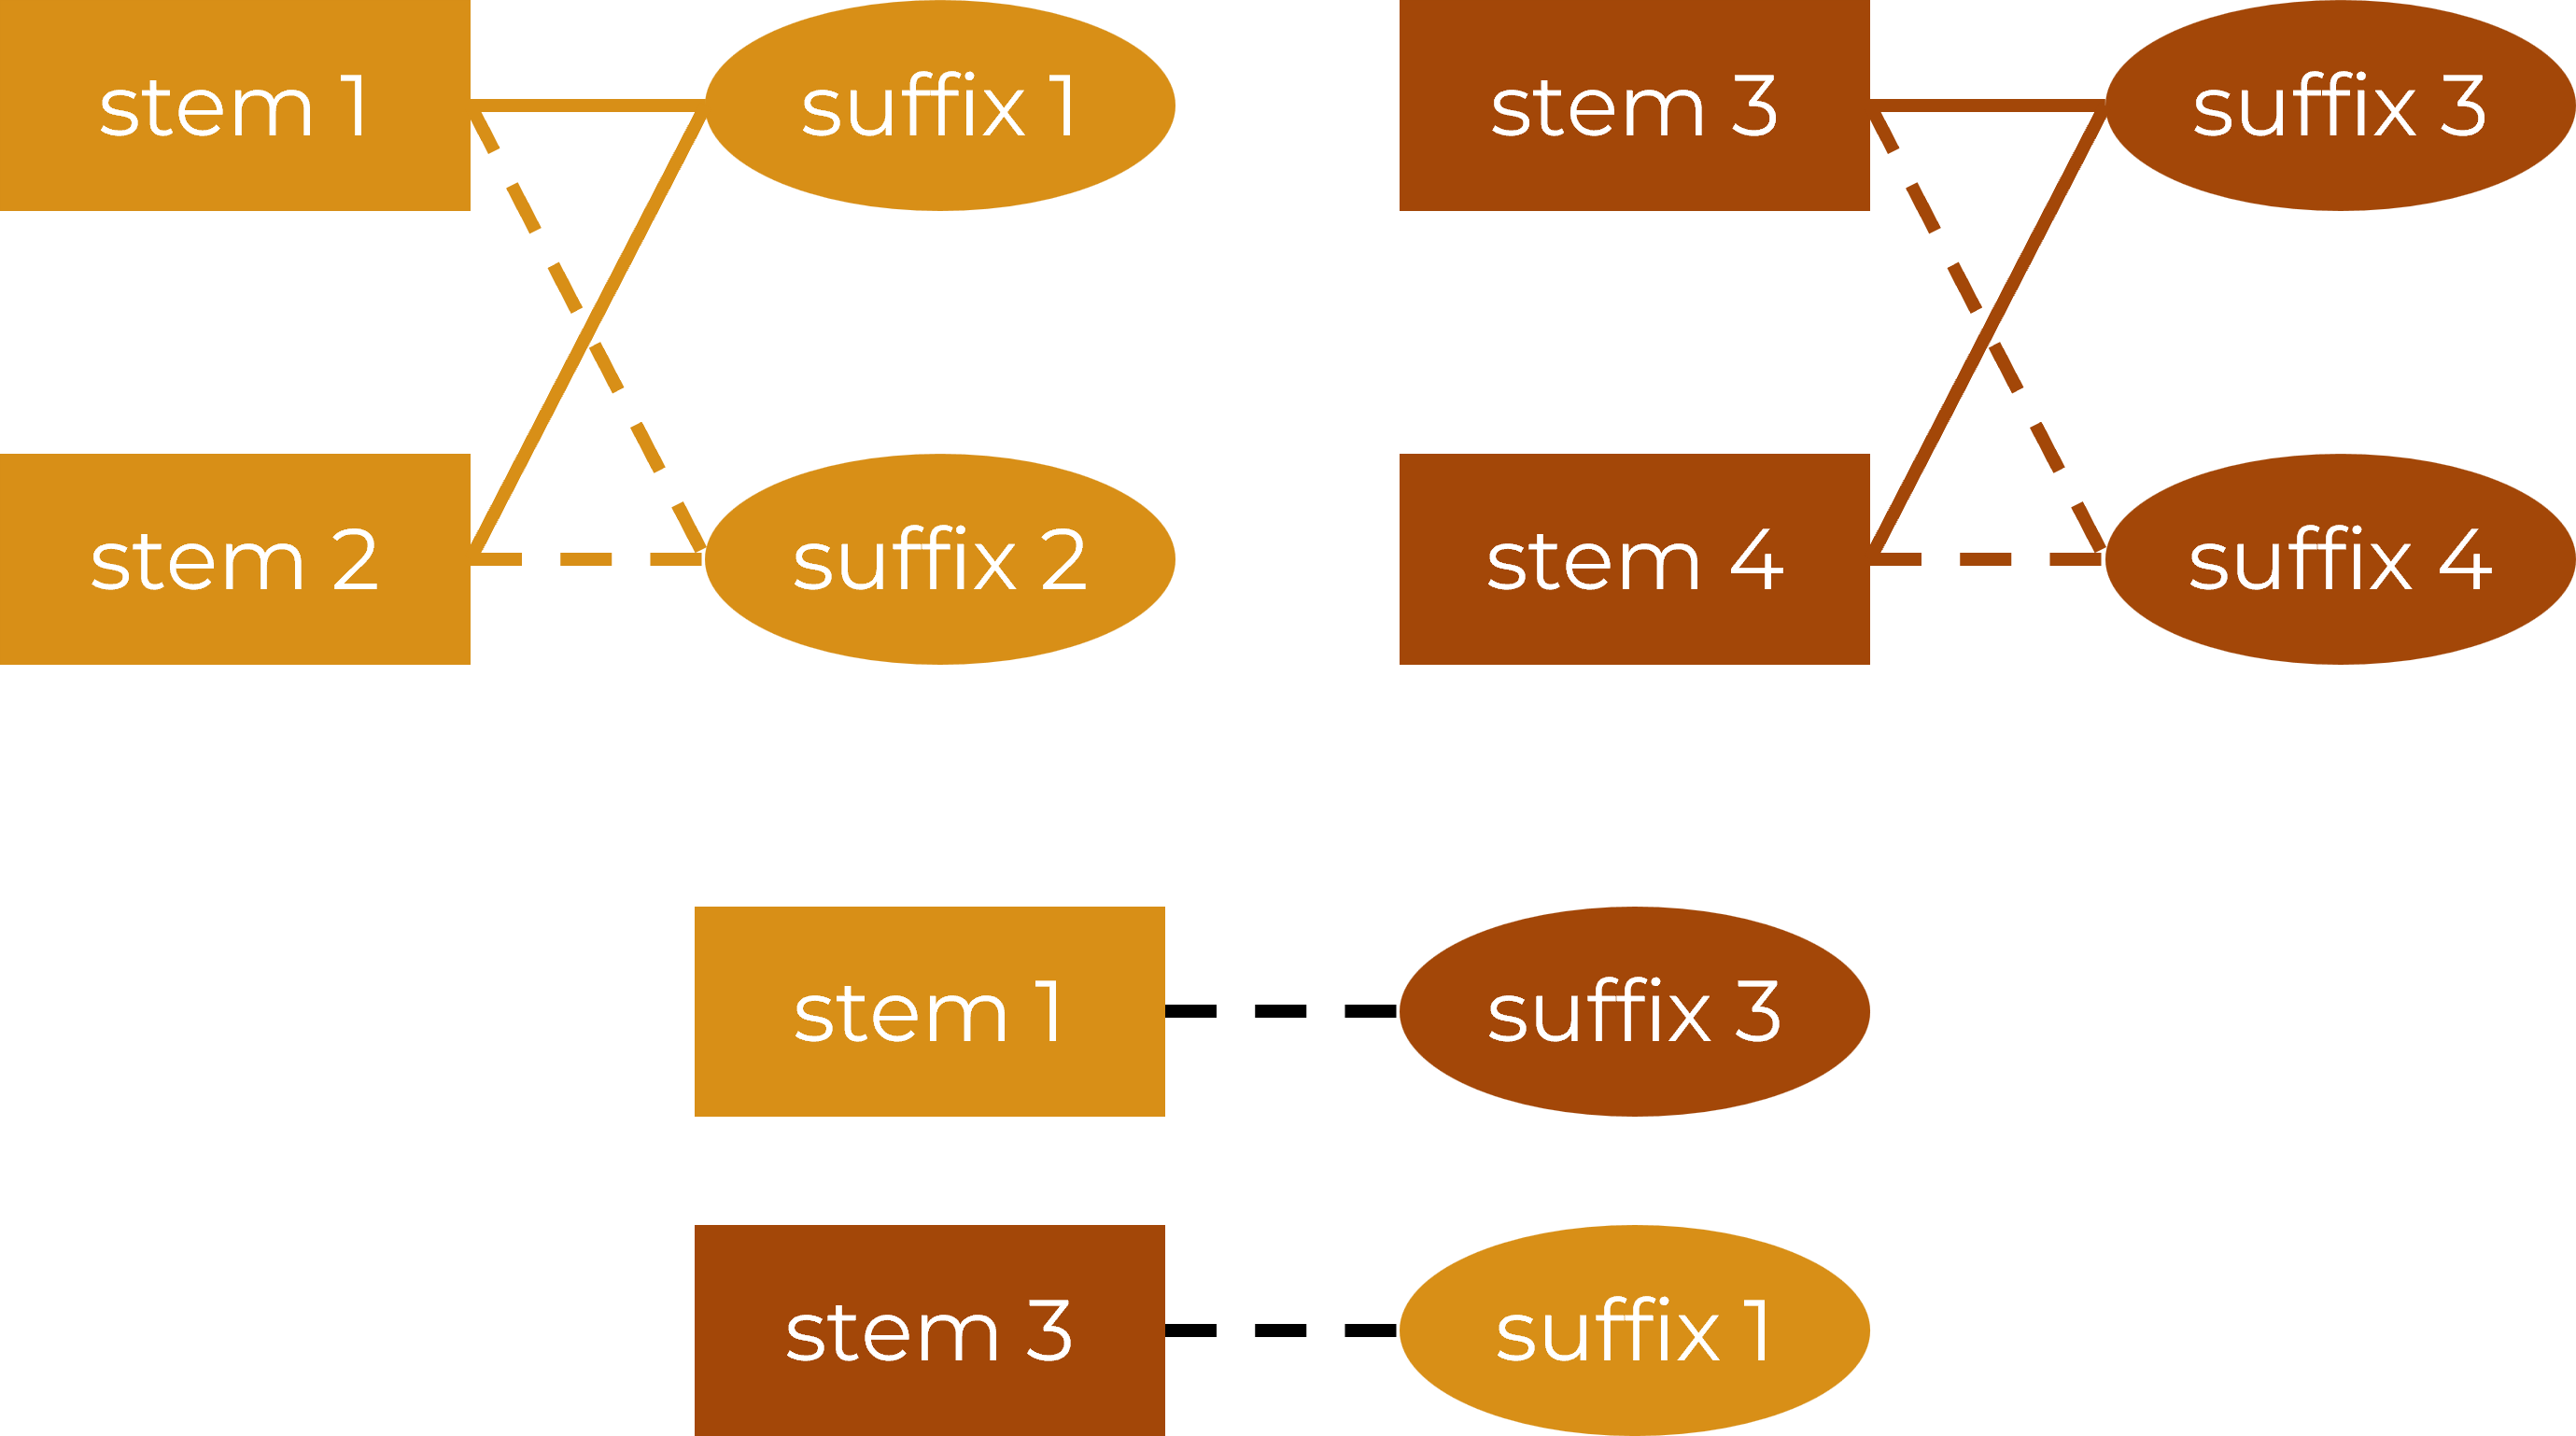
\includegraphics[width=0.6\textwidth]{Figures/Testing_structure.png}
    \end{center}
    \caption[]{\justifying Example of the structure of the training and testing stimuli. In gold: language A, in red: language B. Combinations shown in training are shown by solid connecting lines, and those for testing by dashed connecting lines. This structure is known, for example, by an English-French bilingual. English exposes them to ``sing+ing'' and ``read+ing'', and French gives them ``fin+ir'' and ``chois+ir'', but never ``sing+ir'' or ``chois+ing'': these would seem strange and incompatible with their language experience.}
    \label{Testing_structure}
\end{figure}

Of note is that, for a participant to identify the two language groups, two different flavours of statistical learning need to be deployed. First, the participant needs to recognise re-occurring morphemes within the words and segment each word into its composing morphemes. Next, co-occurrence tracking across word presentations can identify that these morphemes indeed only co-occur with morphemes from one half of the stimulus set, allowing for the classification of the stimuli into two separate language groups. The learned co-occurrence structure therefore acts as an implicit, fully reliable cue as to stimulus category/language.

However, the authors had the additional motivation of attempting to replicate and extend the findings of \textcite{Lelonkiewicz2020}, in which a morpheme familiarity effect was found. In the experiment, participants responded ``yes'' more often to stimuli containing a familiar morpheme than those containing novel chunks. To achieve this in the current experiment, two additional testing conditions were developed, mirroring those in the original paper. In the first, the \textbf{one-morpheme} (``1M'') condition, the morphemes were paired with new random character chunks. These novel chunks were closely matched to the morpheme they replaced. Morpheme position was respected (stems always preceded new chunks, and suffixes were always placed after new chunks), as was chunk length: these had the same number of characters as the morpheme being substituted. Each stem was paired once with a random chunk (stem frequency in 1M = 0.025) and each suffix with 2 different chunks (suffix frequency in 1M = 0.05).

Finally, in the \textbf{zero-morpheme} (``0M'') condition, no morphemes were present. Instead, strings made of two novel character chunks were formed.

\begin{figure}[!htbp]
    \begin{center}
        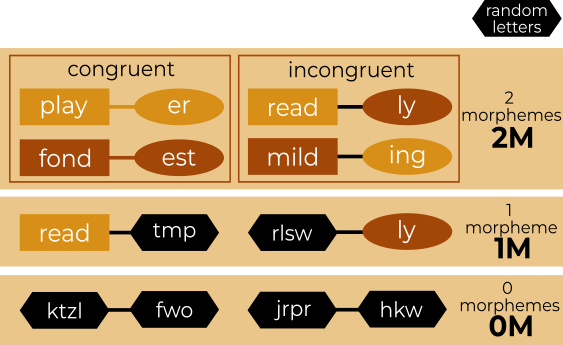
\includegraphics[width=0.6\textwidth]{Figures/testing_conditions.png}
    \end{center}
    \caption[]{\justifying Examples of the structure of testing stimuli in each of the three testing conditions. In gold: language A, in red: language B. In the 2 morphemes (2M) condition, there were novel combinations of same-language (congruent) or different-language (incongruent) morphemes. In the 1 morpheme (1M) condition, the morphemes were combined with novel random strings of letters (black boxes), after \textcite{Lelonkiewicz2020}. In the 0 morphemes (0M) conditions, novel random letter strings were combined together.}
    \label{testing_conditions}
\end{figure}

Overall, there were 40 items in each testing condition. Across all conditions, each stem is shown 3 times (stem frequency = 0.025) and each suffix 6 times (suffix frequency = 0.05).


\noindent \underline{Familiarity test}

\noindent
In order to evaluate participants' degree of learning of the training stream, a familiarity test was devised to test whether segmentation of words into morphemes had occurred. If participants were unable to distinguish congruent from incongruent strings in the 2M condition, but showed good recognition of the original morphemes in the familiarity test, the failure to perform in the 2M condition could safely be attributed to inadequate co-occurrence tracking instead of poor segmentation (in addition to the comparison between the 1M and 0M conditions).

The items for the familiarity test were, on the one hand, all 30 of the morphemes from both languages present in training and, on the other hand, a set of 30 random chunks distinct from those used in the 0M and 1M conditions. The random chunks were matched for length with the morphemes.


\subsubsection{\large{\emph{Procedure}}}
\label{Procedure1}

\noindent \underline{Training}

\noindent
Participants were told that they would be acting as language experts needing to pay attention to words received from an alien transmission. Importantly, none of the instructions contained the words ``language'' or ``languages'' so as to avoid biasing participants towards either the hypothesis that there was a single language set, or that there were multiple. Instead, phrases such as ``the words'' or ``the alien communication'' were carefully chosen to keep this ambiguity: after all, we can't exclude the possibility that, like humans, aliens might speak multiple languages, even within the same population. Participants were then presented with the training words interleaved between both languages, with each word shown once in each of the 8 randomly shuffled training blocks. Each word was presented for 800ms, with 200ms of inter-stimulus interval. Participants were encouraged to take brief breaks between training blocks to avoid fatigue.


\noindent \underline{Testing}

\noindent
Participants were then instructed that they would be reviewing words from a new communication from the same group of aliens, and one from a different group of aliens. They were told that both used the same characters, to avoid participants making judgements on this factor. They were told to be quick to respond, pressing ``d'' or ``k'' in a 2AFC paradigm to indicate whether or not they believed the string being presented belonged to the first group of aliens. In an interleaved order randomised for each participant, strings from all three (0M, 1M, 2M) conditions were shown. Importantly, in order to probe their implicit knowledge rather than letting them form (necessarily unhelpful) visual classification strategies, a timeout of 2 seconds was set for responding to each item. Should a participant spend more time answering, a screen was shown encouraging them to be quicker. Finally, participants were asked which strategy (if any) they used to respond.

\noindent \underline{Familiarity test}

\noindent
Following this, the familiarity test was administered. Similarly to the testing phase, participants had the choice of two keys to select which of the two strings presented was the one they had seen previously in the experiment.

\noindent \underline{Bilingual Language Profile questionnaire}

\noindent
To capture as wide a range of variation within the multilingual population as possible, the Bilingual Language Profile questionnaire (BLP, \textcite{Gertken2014}) was administered. This questionnaire probes language history, use, proficiency, and attitudes, yielding a global language score in a bilingual's languages. It is listed among the most common tests of language dominance (\cite{Olson2023}). Test-retest reliability of the questionnaire with a month between sessions yielded excellent reliability of the difference of global scores in two languages (intraclass correlation = 0.979) and also scores of the individual subsections (history ICC = 0.926; use ICC = 0.960; proficiency ICC = 0.881; attitudes ICC = 0.858 - see \textcite{Olson2023} for full statistics).

To include participants from all geographical regions and allow for free entry of which languages they speak rather than choosing from the list of possible languages in which the BLP has been translated (which, most notably, completely excludes African languages), it was adapted for participants to respond to these questions for up to four languages they may speak, whichever these might be. Additionally, an attention check question was added.



\subsubsection{\large{\emph{Analysis}}}
\label{Analysis1}
\noindent \underline{Pre-processing}

\noindent
Included in the final data sample will be all participants who follow task instructions. Those with a mean response time in testing of over 2 seconds will be excluded, for having replied more on conscious mental strategies over instinctual responses as instructed.

Any data points from testing trials in which the reaction time was inferior to 300ms or superior to 3000ms were excluded from the mixed models analyses.

Participants' BLP subsection and global scores were computed according to the guidelines laid out in \textcite{Gertken2014}.

\noindent \underline{Group-level analyses}

\noindent
In order to evaluate whether the morpheme familiarity effect of \textcite{Lelonkiewicz2020} was replicated in this paradigm, a generalized linear mixed-effects model was fitted to evaluate responses between each testing condition, with estimated marginal means calculated for any significant conditions. For performance in the 2M condition, a simple mixed effects model was run to determine group-level performance. An accuracy score for each participant was also computed by summing the hits and correct rejections of each participant, and d-prime scores were extracted. For familiarity test responses, the percentage of correct responses was used in a Student's t-test.

\noindent \underline{Individual differences analyses}

\noindent
While we strove to deviate from the reductionist tendency to categorise multilinguals according to the number of languages spoken, we also included this variable for the sake of comparison. Based on the 16 scores that that BLP attributes to each participant, we computed the following continuous multilingual metrics.

% Multilingual experience
We used a variable named \textbf{multilingual experience} to quantify how much linguistic exposure a participant has across all of their spoken languages. This was measured by summing up all of a participant's language scores.

% Balance
In continuity with previous research finding language balance to be an important aspect (see \textcite{Gullifer2019}), three measures were elaborated for this construct. \textbf{L1-L2 difference} was a measure of \textbf{bilingual balance}. This was calculated by taking the absolute value of the subtraction of the second language (L2) score from the first language (L1) score. Next, \textbf{language entropy} was used as a measure of \textbf{multilingual balance} that would also consider the effect of eventual third and fourth languages. However, a crucial point in calculating balance is the issue that arises from comparisons between different numbers of languages, so a different number of dimensions of participants' data. Two approaches to resolving this conflict were leveraged. The first, entropy (as in \textcite{Gullifer2019} and \textcite{Onnis2018}), was computed on the overall scores for each language via the \textrm{DescTools} R package's \textrm{entropy} function (\cite{DescTools}). Entropy has the property of applying the same computation to vectors of scores of different lengths. However, a by-product of this is that longer vectors (participants speaking more languages) naturally yield higher entropy scores. As an example, a bilingual speaker with the scores 200 and 200 for their languages has as entropy of 1, while a trilingual speaker with scores of 200, 200, and 200 for their languages receives an entropy score of approximately 1.58, despite both of these profiles showing absolute balance across languages. Entropy might therefore be thought of as a compound measure, considering both multilingual experience and balance.

To untangle multilingual balance from experience, the \textbf{cosine similarity} measure was developed (\autoref{cossim_bi}).

\begin{figure}[!htbp]
    \begin{center}
        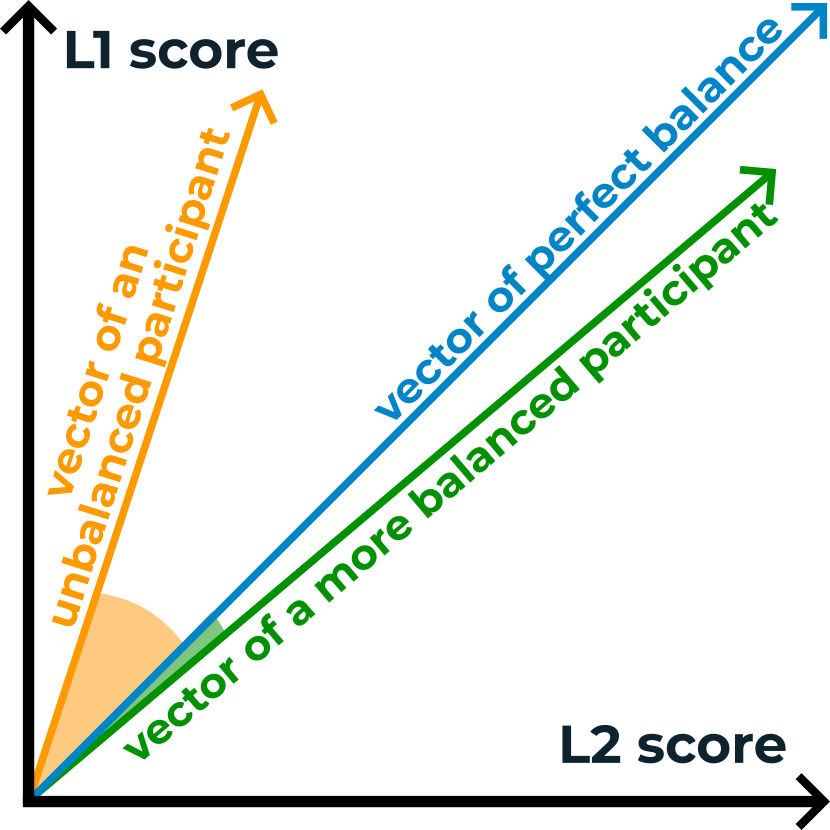
\includegraphics[width=0.4\textwidth]{Figures/cosine_similarity2D.png}
    \end{center}
    \caption[]{\justifying Illustration of the principle of cosine similarity as a measure of language balance. Taking the example of a bilingual participant, one dimension represents the L1 score, with a second dimension for the L2 score. A vector of perfect balance lies in the middle of this two-dimensional plane. Two example participants' language scores are then placed on this plane. First, a participant (in orange) with a high L1 score and low L2 score, is represented as a vector from the origin to the point representing these scores. The angle between this vector and the perfect balance vector is shown in light green. A second example is proposed in green, for a participant with a high L1 score and a slightly higher L2 score. This second participant has a smaller angle to the perfect balance vector, reflecting the closer L1 and L2 scores than in the former example. The same logic can be applied to a higher number of dimensions, which was performed in this study (up to D = 4).}
    \label{cossim_bi}
\end{figure}

Mathematically, with a vector A (the participants' scores vector) and a vector B (the vector of maximal scores):

\centering
$\textrm{cosine similarity} = \frac{A*B}{\vert\vert A\vert\vert * \vert\vert B\vert\vert}$.

\justifying
A participant vector A is defined as $A = (A_1, A_2, A_3, A_4)$, where $A_1$, $A_2$, $A_3$ and $A_4$ are the overall language scores in L1, L2, L3, and L4, respectively.

Importantly, the perfect vector always has as many dimensions as the participant vector. For example, for a bilingual participant ($A = (210, 180)$ for example), $B = (218, 218)$, whereas for a trilingual participant ($A = (210, 180, 180)$), $B = (218, 218, 218)$.

This metric yields a score between 0 and 1, with 0 for vectors with nothing in common (completely dissimilar, a maximally unbalanced participant), and 1 for identical vectors (a perfectly balanced participant). With the current application, the score range is 0.5 to 1, due to the limitations to how dissimilar the two vectors can be provided that the participant score vector is necessarily composed of two non-null positive values.

However, given that participants were able to declare information on up to four spoken languages no matter their proficiency in that language, one participant may choose, for example, to declare very limited knowledge of Japanese. This could consist in knowing a handful of words. Another participant may choose not to declare such a poor understanding of a language. In the case of the first example participant, a very low score would be introduced into the cosine similarity balance calculation, and pull their score far down. This little knowledge of a language is not likely to affect participants in their daily lives. Therefore, to prevent languages with extremely low scores from affecting overall scores, only scores above or equal to 50 (out of 218) were included in cosine similarity calculations.

Naturally, we couldn't be certain a priori that these metrics would describe our participant sample effectively. Therefore, we also adopted a bottom-up approach and ran a Varimax Principal Components Analysis (PCA) including the BLP scores for each section (L1 History, L1 Use, L2 Proficiency, L2 Use, etc.). 

\begin{figure}[!htbp]
    \begin{center}
        \includegraphics[width=0.6\textwidth]{Figures/Exp1_corrplot.png}
    \end{center}
    \caption[]{\justifying Correlation plot of the BLP variables.}
    \label{exp1_corrplot}
\end{figure}

The resulting Principal Components (PCs) were run as predictors in the above linear modelling.

Another aspect of participant background attracted researchers' interest. The script used in each language declared by participants was researched. Participants who were then classified as ``same script'' users for example spoke English and French, both of which use a Latin script. Those who spoke for example English and Greek were ``different scripts'' users.

The metrics were utilised to evaluate individual differences in the morpheme familiarity effect through generalised linear mixed effects models with the following syntax 

\noindent
\begin{center}
    $\textrm{glmer(observed} \sim \textrm{scale(trialn)} + \textrm{testing condition} \ast \textrm{\emph{multilingual variable}} + (1 + \textrm{testing condition } \vert \textrm{ subject ID), family=``binomial'')}$
\end{center}


\noindent
These models were run on all datapoints except those with a response time superior to 300ms and inferior to 3000ms (thereby discarding abnormally short or abnormally long trials).

Mixed effects modelling of 2M performance was achieved through limiting the previous analysis to the 2M condition. In these models, the outcome variable would now be the nature of the strings presented to participants: ``within-language'' or ``between-language'', which are also the options for participant responses:

\noindent
\begin{center}
    $\textrm{participant response} \sim \textrm{scale(trialn)} + \textrm{string nature} \ast \textrm{\emph{variable}} + (1 + \textrm{expected} \vert \textrm{subject ID})$
\end{center}

Finally, further mixed effects modelling observed the effect of the variables on participants' familiarity test score. These models were formulated in the same way as for 2M performance.

All linear modelling was achieved through usage of the lme4 (\cite{Bates2015}) package in R.